\documentclass[12pt]{article}
\usepackage[top=1in, bottom=1in, left=1in, right=1in]{geometry}

\usepackage{setspace}
\onehalfspacing

\usepackage{amssymb}
%% The amsthm package provides extended theorem environments
\usepackage{amsthm}
\usepackage{epsfig}
\usepackage{times}
\renewcommand{\ttdefault}{cmtt}
\usepackage{amsmath}
\usepackage{graphicx} % for graphics files

% Draw figures yourself
\usepackage{tikz} 

% writing elements
\usepackage{mhchem}

\usepackage{paralist}

% The float package HAS to load before hyperref
\usepackage{float} % for psuedocode formatting
\usepackage{xspace}

% from Denovo Methods Manual
\usepackage{mathrsfs}
\usepackage[mathcal]{euscript}
\usepackage{color}
\usepackage{array}

\usepackage[pdftex]{hyperref}
\usepackage[parfill]{parskip}

% math syntax
\newcommand{\nth}{n\ensuremath{^{\text{th}}} }
\newcommand{\ve}[1]{\ensuremath{\mathbf{#1}}}
\newcommand{\Macro}{\ensuremath{\Sigma}}
\newcommand{\rvec}{\ensuremath{\vec{r}}}
\newcommand{\omvec}{\ensuremath{\hat{\Omega}}}
\newcommand{\vOmega}{\ensuremath{\hat{\Omega}}}
%---------------------------------------------------------------------------
%---------------------------------------------------------------------------
\begin{document}
\begin{center}
{\bf NE 155/255, Fall 2019 \\
Simplified Scattering, Diffusion Equation\\
September 20, 2019}
\end{center}

\setlength{\unitlength}{1in}
\begin{picture}(6,.1) 
\put(0,0) {\line(1,0){6.25}}         
\end{picture}

\subsection*{Scattering}
Double differential scattering can be simplified. Let's
start by recalling

\[\Sigma_s(\vec{r}, E', \vOmega' \rightarrow E, \vOmega) =
\Sigma_s(\vec{r},E') f_s(E', \vOmega' \rightarrow E, \vOmega)\:.\]

We can represent the fractional probability as a product of two independent
fractional probabilities (which is technically an assumption, but is
well-supported by reality):

\[f_s(E', \vOmega' \rightarrow E, \vOmega) =
f_{sE}(E' \rightarrow E) f_{s\Omega}(\vOmega'  \rightarrow \vOmega)\:.\]

In the \textbf{monoenergetic} case, $f_{sE}(E \rightarrow E') = 1$ and with
\textbf{isotropic scattering},
$f_{s\Omega}(\vOmega'  \rightarrow \vOmega) = \dfrac{1}{4\pi}$, which would
combine to give
$\Sigma_s(\vec{r}, E', \vOmega' \rightarrow E, \vOmega) =
\dfrac{\Sigma_s(\vec{r})}{4 \pi}$.

If \textbf{scattering is not isotropic}, what do we do? That is, when we can't
simplify so easily, we at least need to represent it in a way we can
numerically manage. There are several approaches; here is one of them. 

We expand the scattering cross section in Legendre Polynomials, which are a
sequence of orthogonal polynomials:

\[P_n(x) =
\frac{1}{2^n n!}\frac{d^n}{dx^n} \bigl[\bigl( x^2 -1 \bigr)^n\bigr]\:,\]

as follows

\[\Sigma_s(\vOmega' \cdot \vOmega) =
\sum_{l=0}^{\infty} \frac{2l+1}{4\pi} \Sigma_{sl} P_l(\mu_0) =
\sum_{l=0}^{\infty} \frac{2l+1}{4\pi} \Sigma_{sl} P_l(\vOmega')P_l(\vOmega)
\:. \]

Note that we used the Legendre Addition Thoerem, which uses spherical 
harmonics. For now, just note that there are identities and manipulations that 
allow this to be true. 

Legendre polynomials are solutions to Legendre's differential equations,

\[\frac{d}{dx}\bigl[(1 - x^2) \frac{d}{dx} P_n(x) \bigr] +
n(n+1)P_n(x) = 0\:,\]

and are orthogonal on $[-1,1]$:

\begin{gather*}
\int_{-1}^{1}P_n(x)P_m(x)dx = 
\frac{2}{2n+1}\delta_{n,m}= \quad\frac{2}{2n+1}\text{if n = m,} 
\quad 0\text{ if n $\neq$ m.}\\
\therefore P_0(\mu) = 1 \\
P_1(\mu) = \mu\:.
\end{gather*}

We can see the first several polynomials in \autoref{fig:legendre}.

\begin{figure}[h!]
    \begin{center}
    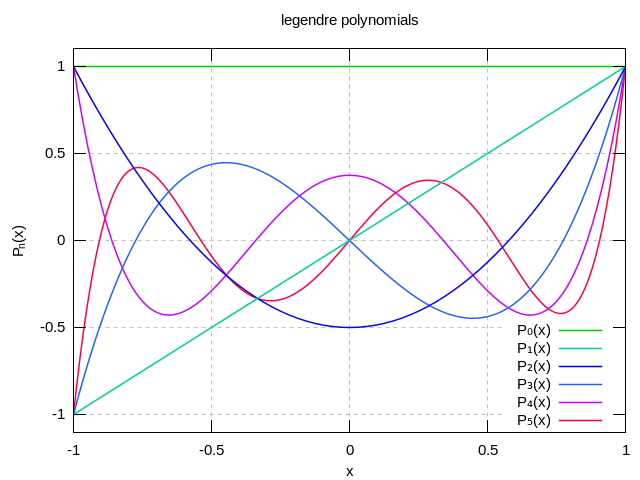
\includegraphics[keepaspectratio, width = 3.5 in]{Legendrepolynomials}
    \end{center}
    \caption{Legendre polynomials.}
    \label{fig:legendre}
    %https://en.wikipedia.org/wiki/Legendre_polynomials
\end{figure}

We get the scattering expansion coefficients from the orthogonality of
Legendre Polynomials. Any function can be expanded on the interval
$-1 \leq x \leq 1$

\[
f(x) = \sum_{n=0}^{\infty} \frac{2n+1}{2} f_n P_n(x)
\]

To find $f_n$, multiply by $P_l$ and integrate over $(-1,1)$:

\begin{align*}
\int_{-1}^1 dx\: f(x) P_l(x) &=
\sum_{n=0}^{\infty} \frac{2n+1}{2} f_n\int_{-1}^1 dx\:  P_n(x) P_l(x)\\
\therefore f_n &= \int_{-1}^1 dx\: f(x) P_l(x)\\
\text{and by analogy}\Sigma_{sl} &=
2\pi \int_{-1}^1 d\mu_0 \: P_l(\mu_0)\Sigma_s(\mu_0)\:.
\end{align*}

All of that was to say, we can actually deal with scattering when it's
\textit{not} isotropic by expressing the scattering cross section as an
expansion in Legendre polynomials. In our simplified transport equation, this
looks like:

\begin{align*}
\mu \frac{\partial \psi(z, \mu)}{\partial z} &+ \Sigma_t(z)\psi(z, \mu) = \\
&\frac{\nu\Sigma_f(z) }{2}\phi(z) +
\sum_{l=0}^{\infty} \frac{2l+1}{2} \Sigma_{sl}(z) \int_{-1}^1 d\mu'\:
P_l(\mu_0) \psi(z, \mu')  + \frac{S(z)}{2} \:.
\end{align*}

In reality, we truncate the expansion at some point. Some common truncations:

\begin{align*}
&l=0 \text{ is isotropic; (note } P_0 (\vOmega) = 1 \text{)}\\
&\qquad \Sigma_s(\vOmega' \cdot \vOmega) \cong \frac{1}{4\pi}\Sigma_{s0} \\
%
&l=1 \text{ is linearly isotropic; (note } P_1 (\vOmega) = \vOmega \text{)}\\
&\qquad \Sigma_s(\vOmega' \cdot \vOmega) \cong
\frac{1}{4\pi}\bigl( \Sigma_{s0} + 3\vOmega' \vOmega \Sigma_{s1} \bigr) 
\end{align*}

In describing representations of the TE, people commonly describe the
scattering by saying the ``$P_n$'' expansion of scattering. 

%-------------------------------------------------------------
\subsection*{Diffusion Equation}

The \underline{diffusion approximation} is a widely used simplification that
reduces the computational complexity of the transport equation. 

The approximation is that the \textbf{angular dependence of the flux is unimportant},
so the direction component of the transport equation can be discarded.
Physically this means that neutrons move against their concentration gradient
like just heat diffuses through a conductor. 

The information in this section is derived from Duderstadt and Hamilton's
\emph{Nuclear Reactor Analysis} and neglects fission for simplicity. 

The first step in applying this approximation is to integrate the angular
dependence out of the transport equation, resulting in the neutron continuity equation:
%
\begin{equation}
  \nabla \cdot J(\vec{r},E) + \Macro(\vec{r},E)\phi(\vec{r},E) = \int \:dE' \:\Macro_{s}(\vec{r}, E' \to E)\phi(\vec{r},E') + Q_{ex}(\vec{r},E) \:,
  \label{eq:continuity} 
\end{equation}
%
where the following definitions have been used:
%
\begin{itemize}
\item $J(\vec{r},E) = \int d\vOmega \:\vOmega \psi(\vec{r}, \vOmega, E)$ is the neutron current \\
\item  $\phi(\vec{r},E) = \int d\vOmega \:\psi(\vec{r}, \vOmega, E)$ is the scalar flux, and \\
\item $Q_{ex} (\vec{r},E)= \int d\vOmega \:q_{ex}(\vec{r}, \vOmega, E)$ is the external source.
\end{itemize}

Unfortunately, this simplifying approximation added another unknown, $J$,
which leaves one equation with two unknowns. 

In an attempt to eliminate one of these unknowns, Equation
\eqref{eq:continuity} is multiplied by $\hat{\Omega}$ and integrated over angle
again to obtain the first angular moment:
%
\begin{align}
  \nabla \cdot \int  d\vOmega \:\vOmega \vOmega \psi(\vec{r}, \vOmega, E) &+ \Macro(\vec{r},E) J(\vec{r},E)= \nonumber \\
  &\int dE' \:\Macro_{s1}(\vec{r}, E' \to E)J(\vec{r},E') + \int d\vOmega \int d\vOmega \:\vOmega q_{ex} \:,
  \label{eq:current1}
\end{align}
%
where $\Macro_{s1}  = \int d\vOmega \:\vOmega \Macro_{s}$. The first angular moment form of the equation cannot be solved either because the streaming (first) term is still unknown. 

To make Equation \eqref{eq:current1} solvable, the original assumption is modified to assert that the angular flux is weakly, in fact \textbf{linearly, dependent on angle rather than independent of angle}.

To implement this assumption the angular flux is expanded in angle and only the first two terms are retained:  
%
\begin{equation}
  \psi(\vec{r}, \vOmega, E) \cong \frac{1}{4 \pi} \phi(\vec{r}, E) + \frac{3}{4 \pi}J(\vec{r}, E) \cdot \vOmega \:.
  \label{eq:angExpand} 
\end{equation}

The truncated angular flux is then inserted into the streaming term in Equation \eqref{eq:current1}, giving 
%
\begin{equation}
  \nabla \cdot \int d \vOmega \:\vOmega \vOmega \psi(\vec{r}, \vOmega, E)  \cong \frac{1}{3} \nabla \phi(\vec{r}, E) \:. 
  \label{eq:firstTerm}
\end{equation}


\end{document}
